\begin{figure}
   \begin{minipage}[b]{0.55\columnwidth}
    \centering
       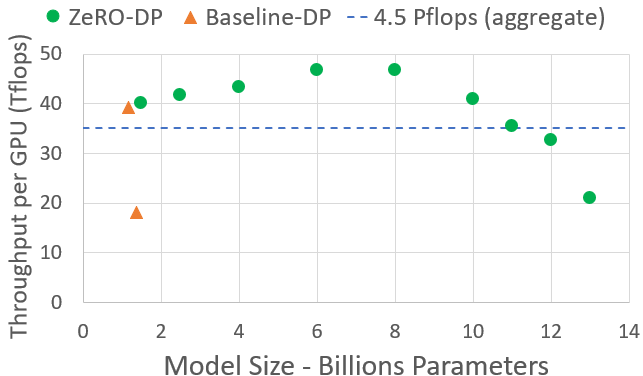
\includegraphics[width=\textwidth]{max_data_parallel_throughput.PNG}
        \caption{Max model throughput with \name-DP.} \label{fig:dp_tput}
   \vspace{0.04in}
   \end{minipage}
%   \vspace{-0.13in}
    \quad
   \begin{minipage}[b]{0.4\columnwidth}
    \centering
       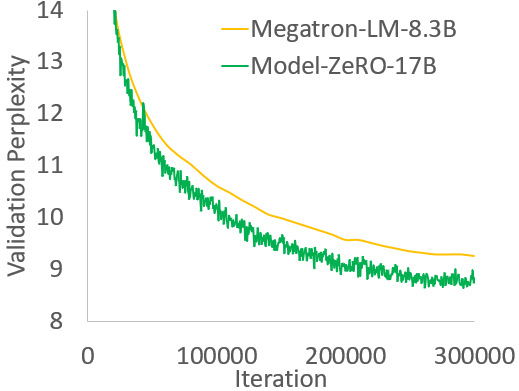
\includegraphics[width=\textwidth]{turing_nlg_17B.PNG}
        \caption{SOTA Turing-NLG enabled by \name.} \label{fig:turing_nlg_17B}
      \vspace{0.08in}
   \end{minipage}
\end{figure}
\section{Implementation and Evaluation}\label{sec:evaluation}

We focus our implementation on supporting efficient training of models with {$\sim$}100B parameters, which are an order-of-magnitude larger than the largest published models today (e.g., T5-11B~\cite{T5}) while trainable within a reasonable time frame on current hardware (e.g., with 1K V100 GPUs).  We implement and evaluate a subset of optimizations in \name --- $P_{os+g}$ in \name-DP plus ZeRO-R --- that allows us to achieve this goal. We will refer to this implementation as \name-100B.  Our results show that \name-100B can efficiently train models with up to 170B parameters, 8x bigger than SOTA, up to 10x faster and with improved usability. \name-100B powers Turing-NLG, the largest published model in the world with new SOTA accuracy.   

%Here, we demonstrate the performance of \name for models with up to 170B parameters. We show that \name-100B achieves better than perfect scalability in the regime that we tested. We show how \name democratizes large model training by providing data scientist the freedom to experiment without constraints, and making large model training feasible on lower end clusters. Furthermore, we discuss the impact of different optimization in \name-100B on model size, memory consumption and performance. We also present the \name-100B powered Model-\name, a 17.2B parameter transformer based model which is not only the SOTA for language models but is also the largest model in the world. We begin by presenting a brief discussion of our implementation and methodology.

\begin{table}
\centering
   \begin{minipage}[b]{0.30\columnwidth}
       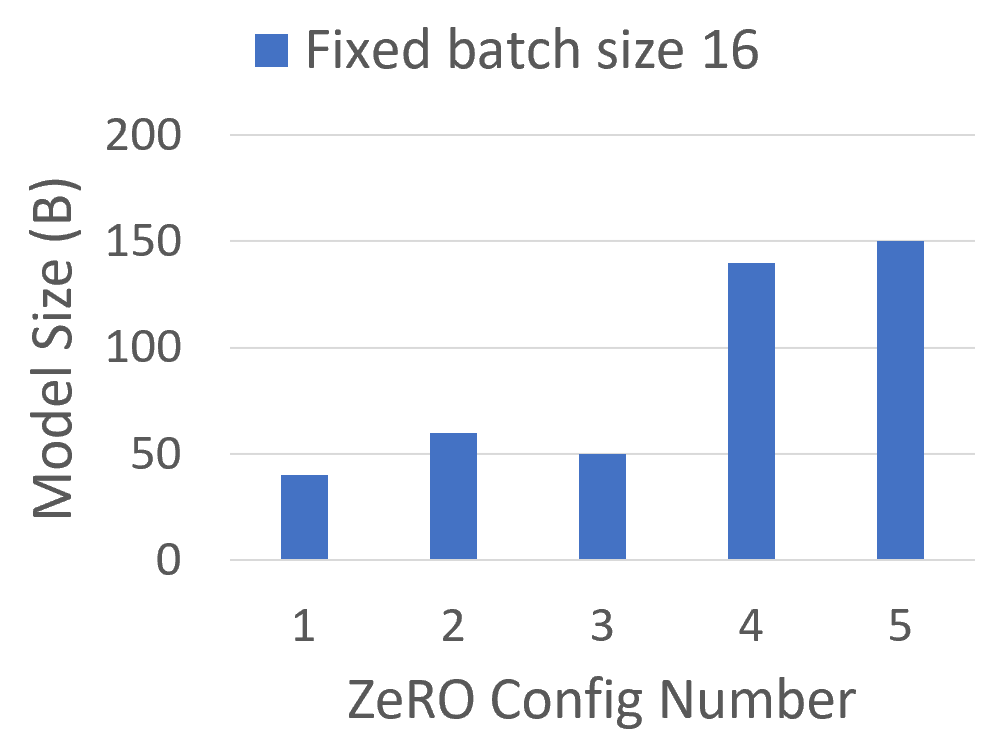
\includegraphics[width=\textwidth]{max_model_size.PNG}
        \captionof{figure}{Max model size \vspace{2pt}}. \label{fig:max-model-size}
   \end{minipage}    
   \quad
   \begin{minipage}[b]{0.30\columnwidth}
       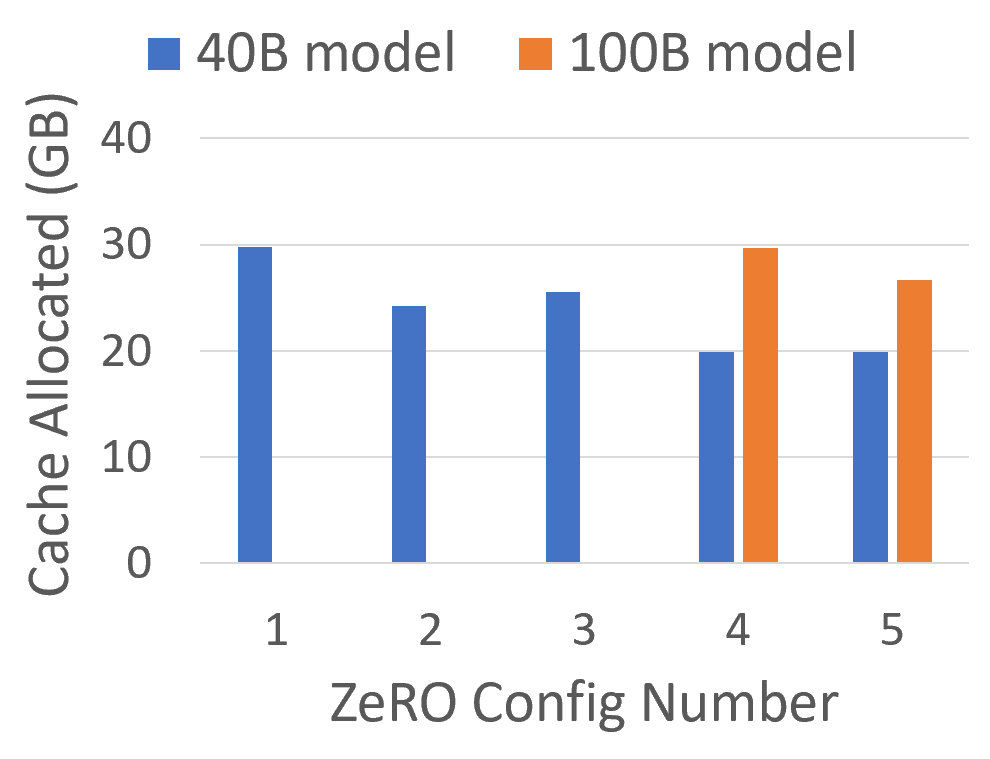
\includegraphics[width=\textwidth]{cache_allocated.PNG}
       \captionof{figure}{Max cache allocated.} \label{fig:max-cached-memory}
   \end{minipage}    
   \quad
   \begin{minipage}[b]{0.30\columnwidth}
       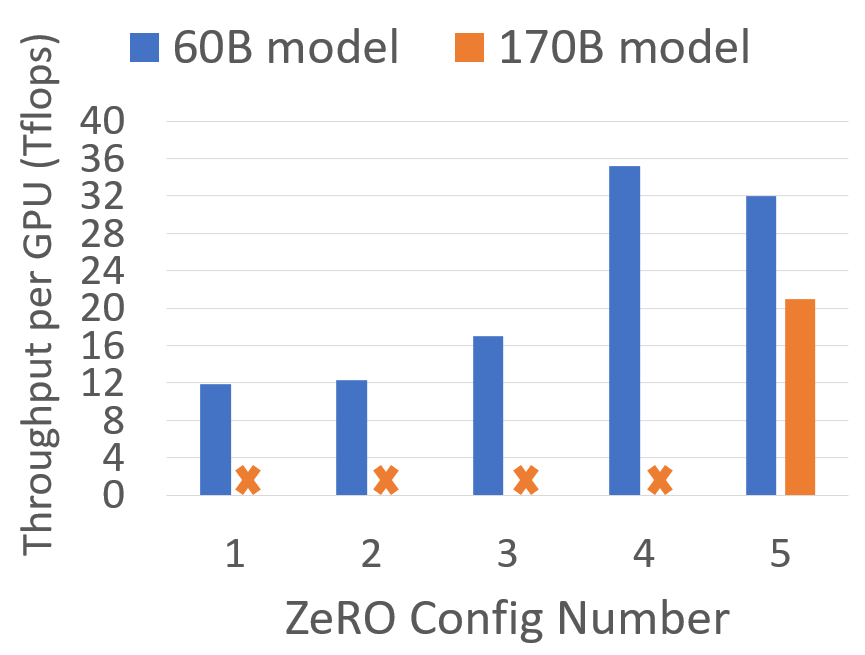
\includegraphics[width=\textwidth]{tput_vs_config.PNG}
        \captionof{figure}{\small{Throughput per GPU}.} \label{fig:max-performance}
   \end{minipage}
   \end{table}
  
\subsection{Implementation and Methodology}

%\paragraph{\name and MP} 

\paragraph{Implementation}
We implemented \name-100B in PyTorch including the full set of optimizations in $P_{os+g}$ and \name-R.  Its interface is compatible with any model implemented as an {\tt torch.nn.module}. Users can simply wrap their models using this interface and leverage \name-powered DP as they use classic DP. Users do not need to modify their model.  \name-powered DP can be combined with any form of MP including Megatron-LM.

\paragraph{Hardware}
We conducted our experiments on a cluster of 400 V100 GPUs ($25$ DGX-2 nodes) with 800 Gbps internode communication bandwidth.
%Details of our hardware environment are summarized in Table~\ref{tab:hardware_environment}. 

\paragraph{Baseline}
For experiments without MP, we use torch's distributed data parallel (DDP) as baseline. For experiments with MP, we use Megatron-LM because it is, to our knowledge, the state-of-art. We use the open-source version of Megatron-LM from NVIDIA~\footnote{https://github.com/nvidia/Megatron-LM} with a date of September 2019. The most recent Megatron-LM results report the ability to scale up to 16B parameter models using 32 DGX-2 nodes (total of 512 32GB V100 GPUs) \cite{megatronlm}. %Megatron-LM also comes with its own data-parallel implementation.

\paragraph{\name}
Experiments without MP, use the \name-powered DP implementation in \name-100B. 
%As discussed in Sec.~\ref{sec:intro}, \name can be combined with MP to achieve a multiplicative effect in memory reduction. We use \name in conjunction with MP to efficiently train very large model sizes. 
Experiments with MP, combine \name-powered DP with MP of Megatron-LM.

\paragraph{Model Configurations}
The models presented in this section are GPT-2 \cite{gpt-2} like transformer based models. We vary the hidden dimension and the number of layers to obtain models with different number of parameters. Table~\ref{tab:model-configuration} shows the configuration parameters used in our experiments with additional details in AE Appendix.

\begin{comment}
While 1T parameter model requires exa-flop supercomputers, 80B-100B parameter models may be trained in a few weeks on a 1024 GPU system which already exists (once again assuming the same sequence length and data size, and similar computational efficiency). As such, for the first step of the evaluation, we implemented optimizer state partitioning ($P_{os}$) and demonstrated its capability to support such models, which would hopefully address the near-term growth on model size.  We call this implementation \nameos.   The full implementation of \name and its support for trillion parameters will come later.  

\subsection{\nameos Implementation}
We implemented \nameos for PyTorch as a wrapper class of torch optimizer. To use \nameos, torch users can simply swap out their favourite optimizer with \name wrapped version of the same optimizer, requiring just a few lines of code change.

\nameos implements $P_{os}$ to eliminate optimizer state redundancy, and $C_B$ to reduce the all-reduce buffer sizes. The all-gather required by $P_{os}$ can be performed either as all-gather or as a sequence of broadcast operations. 
The former has less latency impact, but the later has less memory overhead (using smaller buffers).  
%The latter has much lower memory overhead, and is handy to avoid running out of memory when running largest trainable models with $P_{os}$.

\nameos incurs 1.5x communication volume compared to baseline data-parallel, as we are currently using all-reduce instead of reduce-scatter. 
It is straightforward to eliminate the additional communication by switching to reduce-scatter.
We observe when the batch size per device is moderate (e.g., 16), this 1.5x of communication volume is not really a bottleneck.
%But even with 1.5x overhead, communication is not really a bottleneck on our systems. 
It also serves the purpose of emulating the communication volume when we enable all optimizations $P_{os + g + p}$ for \name.
%, the 1.5x communication volume is less of a concern for system scalability.

%In fact, while it is straight forward to avoid the communication overhead by switching to reduce-scatter, we used all-reduce on purpose to demonstrate that even with 1.5x communication overhead, communication is not a major bottleneck on the current generation state-of-art hardware systems. This demonstrates the practical value of $P_{os + g + p}$ for \name-1T, when capacity becomes available.


\begin{figure*}
   \centering
   \begin{minipage}[b]{0.3\textwidth}
       \centering
       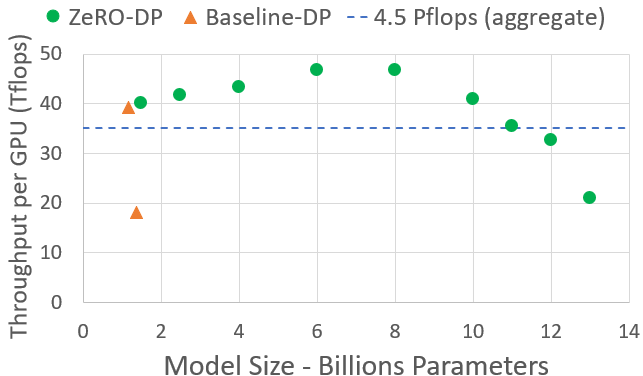
\includegraphics[width=\textwidth]{max_data_parallel_throughput.PNG}
        \caption{Max \name throughput with data parallelism only. \label{fig:dp_tput}}
   \end{minipage}
   \quad
   \begin{minipage}[b]{0.65\textwidth}
   \centering
   \begin{subfigure}[b]{0.3\textwidth}
       \centering
       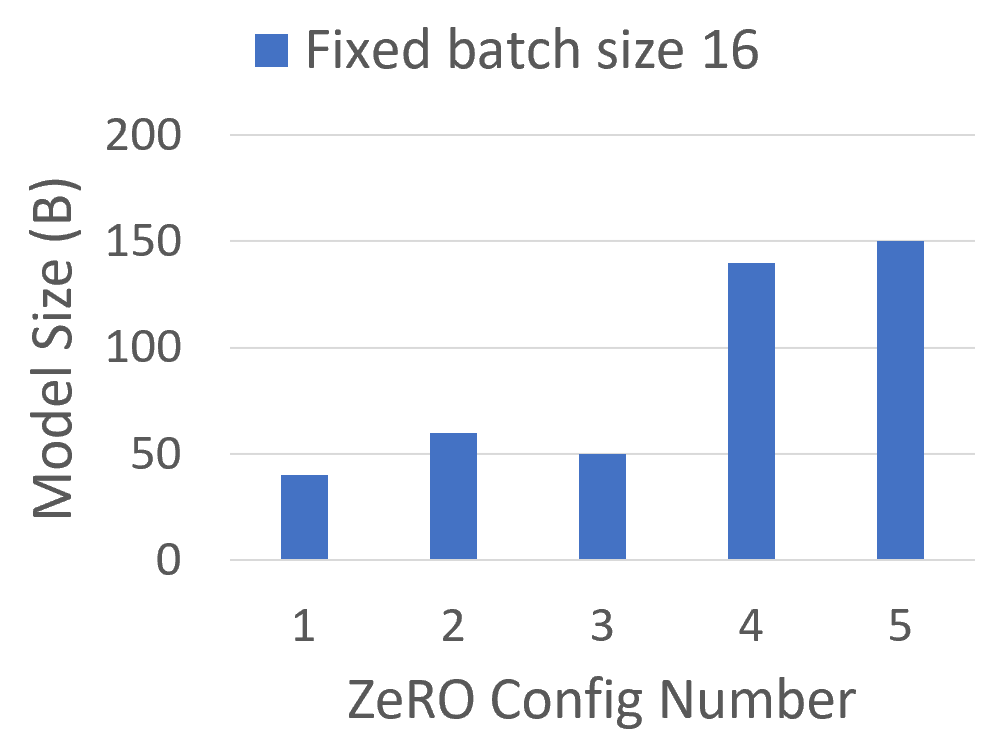
\includegraphics[width=\textwidth]{max_model_size.PNG}
        \caption{Max model size. \label{fig:max-model-size}}
   \end{subfigure}
   \quad
   \begin{subfigure}[b]{0.3\textwidth}
       \centering
       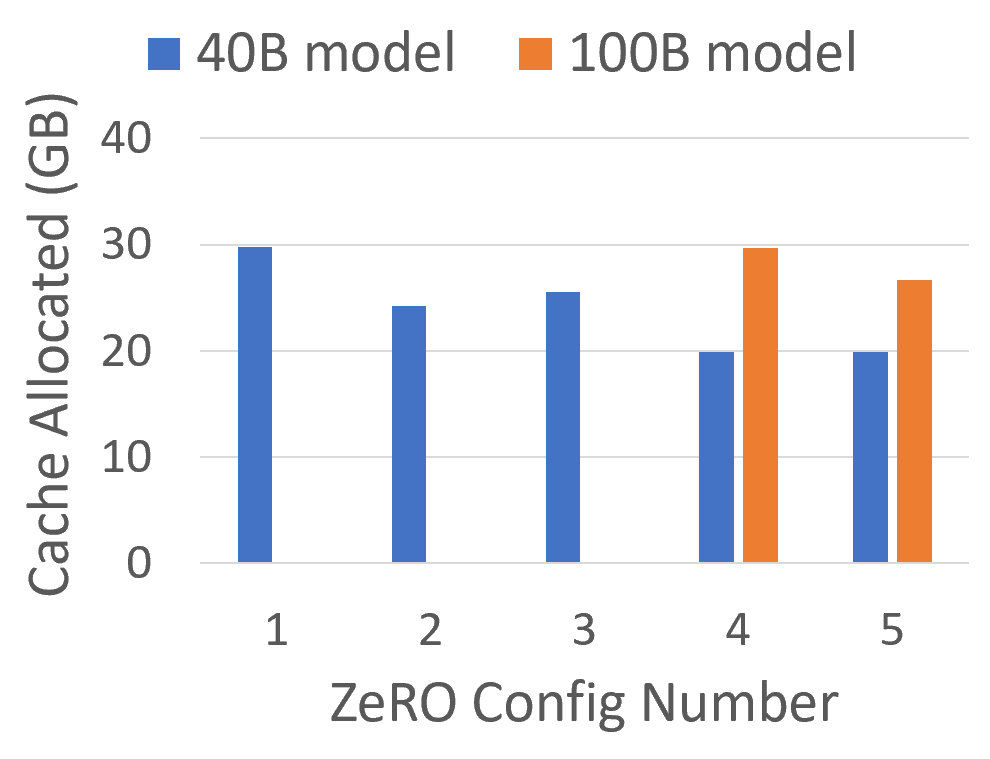
\includegraphics[width=\textwidth]{cache_allocated.PNG}
       \caption{Max cache allocated. \label{fig:max-cached-memory}}
   \end{subfigure}
   \quad
   \begin{subfigure}[b]{0.3\textwidth}
       \centering
       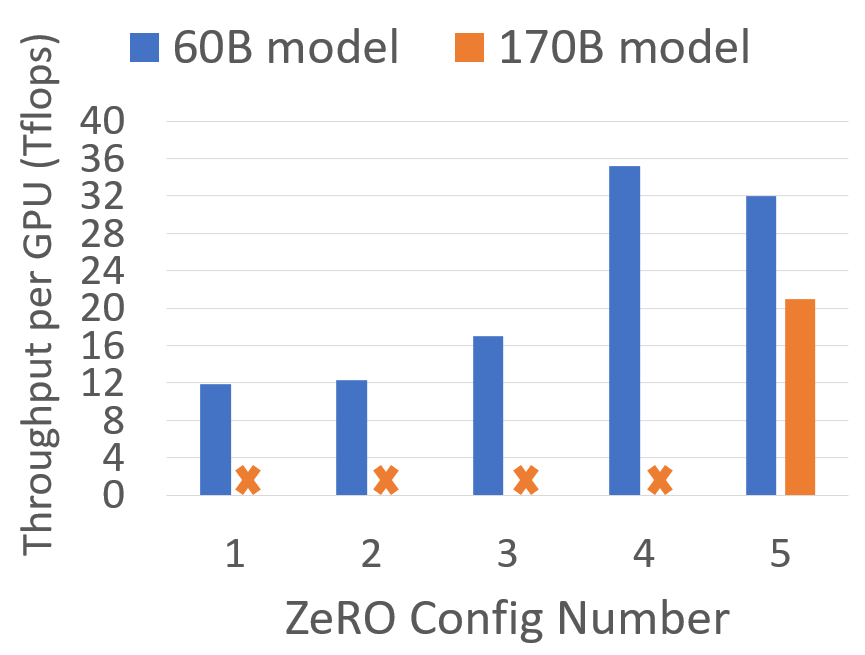
\includegraphics[width=\textwidth]{tput_vs_config.PNG}
        \caption{Throughput per GPU. \label{fig:max-performance}}
   \end{subfigure}
   \caption{Comparing ZeRO configurations.} \label{fig:zero-config-compare}
   \end{minipage}
\end{figure*}
\end{comment}

\subsection{Speed and Model Size}
\name-100B efficiently run models with up to 170B parameters on 400 GPUs, more than 8x bigger than Megatron-LM. Figure~\ref{fig:billion_parameter_speedup} shows throughput per GPU for varying model sizes using \name-100B with MP versus using Megatron MP alone. \name-100B achieves a sustained throughput of 15 PetaFlops (over 30\% of the peak) on average for models with 8B to 100B parameters. In comparison, the baseline MP performance degrades quickly with the increase in model size: MP incurs high communication volume between GPUs, and going beyond a single node to fit larger models causes a communication bandwidth drop from 300GB/sec per link (NVSwitch) to 12.5 GB/sec per link (Infiniband EDR), resulting in a significant performance drop. \name-100B achieves up to 10x speedup over baseline, significantly outperforming on large models.

For \name-100B, the slight reduction in performance beyond 100B is due to lack of enough memory to run larger batch sizes. We expect the performance to improve as we increase the number of GPUs due to super-linear speedup of \name-100B as we discuss next. 
\begin{table}\centering
         \begin{tabular}{|c|c|c|}
         \hline
         & \name-DP & \name-R \\
         \hline
         1 & P$_{os}$&C$_{B}$+M$_{D}$\\
         \hline
         2 & P$_{os}$&C$_{B}$+M$_{D}$+P$_{a}$\\
         \hline
         3 & P$_{os+g}$&C$_{B}$+M$_{D}$\\
         \hline
         4 & P$_{os+g}$&C$_{B}$+M$_{D}+$P$_{a}$\\
         \hline
         5 & P$_{os+g}$&C$_{B}$+M$_{D}$+P$_{a+cpu}$\\
         \hline
         \end{tabular}
     \caption{\name configurations}\label{tab:Opt-table}

\end{table}
\subsection{Super-Linear Scalability}
\name-100B demonstrates super-linear scalability for very large model sizes. Figure~\ref{fig:hyperscale_60B} shows scalability results for a 60B parameter model going from 64 to 400 GPUs and we expect this trend to continue further for more GPUs. $P_{os+g}$ reduces per GPU memory consumption of \name-100B with increase in DP degree, allowing \name-100B to fit larger batch sizes per GPU\footnote{Increasing batch size too much can lead to poor convergence, but for these large models, we are still in a regime where batch size is small enough even with 1K GPU and it does not affect convergence rate}, which in turn improves throughput as a result of increasing arithmetic intensity. 
%We realize that these results do not represent strong or weak scaling in the traditional sense. However, in practical terms, this scaling directly corresponds to the end-to-end wall-clock time which is the most meaningful metric to evaluate scalability for DL workloads.


% \begin{table}[]
% \begin{tabular}{|l|l|c|l|l|c|}
% \hline
% \multicolumn{3}{|c|}{Figure ~\ref{fig:billion_parameter_speedup}} & \multicolumn{3}{c|}{Figures ~\ref{fig:hyperscale_60B}, \ref{fig:dp_tput}} \\ \hline
% \multicolumn{1}{|c|}{} & \multicolumn{1}{c|}{Layers} & HD & \multicolumn{1}{c|}{} & \multicolumn{1}{c|}{Layers} & HD \\ \hline
% 1.5B & 48 & 1600 & 1.16B--2.5B & 24,34,54 & 1920 \\ \hline
% 8B & 72 & 3072 & 4B & 64 & 2304 \\ \hline
% 20B & 98 & 4096 & 6B-8B & 52,72 & 3072 \\ \hline
% 40B--60B & 88, 132 & 6144 & 10B--13B & 50,54,58,62 & 4096 \\ \hline
% 80B--170B & \begin{tabular}[c]{@{}l@{}}100,125,150,\\ 175,212\end{tabular} & 8192 & 60B & 75 & 8192 \\ \hline
% \end{tabular}
% \caption{Configurations for different model sizes, number of layers, and hidden dimensions (HD) across Figures~\ref{fig:billion_parameter_speedup}, \ref{fig:hyperscale_60B}, \ref{fig:dp_tput}.} \label{tab:model-configuration}
% \vspace{-0.10in}
% \end{table}

\subsection{Democratizing Large Model Training}
Using MP and PP is challenging for many data scientists, which is a well-known hurdle to train large models.  \name does not require any changes to the model itself and it can be used as simple as baseline DP while delivering significantly boosted model size and speed.  Fig.~\ref{fig:dp_tput} shows that \name-100B can train models with up to 13B parameters without MP on 128 GPUs, achieving throughput over 40\,TFlops per GPU on average. In comparison, without \name, the largest trainable model with DP alone has 1.4B parameters with throughput less than 20\,TFlops per GPU. 
Furthermore, in the absence of the communication overhead from MP, these models can be trained with lower-end compute nodes without very fast intra-node interconnect such as NVLINK or NVSwitch, which is required to achieve good efficiency with MP.  
%In fact, \name-100B enables a 10B model to train faster than the fastest model using DP alone, which was a 1.2B parameter model running at 39 TFlops per GPU based on our experiments. 

%With \name-100B, the largest models in literature, the T5 11B \cite{T5} and Megatron 8.3B \cite{megatronlm} can be efficiently trained without any form of MP or PP. This allows data scientist can experiment freely with large model sizes because unlike MP or PP, \name does not require any changes to the model itself. 

\subsection{Memory and Performance Analysis}
We look into the benefits and impact of different optimizations on maximum model size, memory consumption and performance. These optimizations are referred to as Config 1 to 5 (C1-C5) in Table.~\ref{tab:Opt-table}.

%present insights into the optimizations in \name-100B by demonstrating the impact of \name-DP (namely $P_{os}$ and $P_{os+g}$), \name-R and \name-R with CPU off-loading($P_{a+cpu})$ on maximum model size, memory consumption and performance. There optimizations are referred to as Config 1 though 5 (C1-C5) as shown in Table.~\ref{tab:Opt-table}.
\paragraph{Maximum Model Size}
Figure~\ref{fig:max-model-size} shows the largest trainable model by enabling different \name optimizations for a fixed batch size and MP of 16. The model size increase from 40B to 60B when trained with C1 vs C2  due to a 16x (MP degree) reduction in activation memory from using $P_a$, while the jump to 140B using C4 is from enabling $P_{os+g}$ which halves the memory requirement by the model states compared to $P_{os}$ in C2. The increase to 150B using C5 is solely due to further reduction in activation memory from offloading the partitioned activation checkpoints to the CPU memory.
\paragraph{Max Cached Memory}
Figure~\ref{fig:max-cached-memory} shows the maximum memory cached by PyTorch during each training iteration for a 40B and a 100B parameter model. The decrease of the cached memory size is as expected from C1 to C2. The difference in memory consumption between C2 and C3 depends on the size of the model states in comparison to the activation memory, and can increase when activation memory is larger, or decrease when the model states are larger. It is note worthy that the cached memory does not decrease from C4 to C5 for 40B but it does for 100B. This is simply because the activation memory for 100B is much larger for the decrease to be noticeable. This makes $P_{a+cpu}$ a valuable tool to fit a larger batch size when we get to very large models. In Figure~\ref{fig:max-performance}, $P_{a+cpu}$ is needed for 170B model to execute without running out of memory.

\begin{table}[]
\centering
\begin{tabular}{|l|l|l|l|l|l|}
\hline
\multicolumn{3}{|c|}{Figure ~\ref{fig:billion_parameter_speedup}} & \multicolumn{3}{c|}{Figures ~\ref{fig:hyperscale_60B}, \ref{fig:dp_tput}} \\ \hline
\multicolumn{1}{|c|}{} & \multicolumn{1}{c|}{Layers} & \multicolumn{1}{c|}{HD} & \multicolumn{1}{c|}{} & \multicolumn{1}{c|}{Layers} & \multicolumn{1}{c|}{HD} \\ \hline
1.5B      & 48          & 1600 & 1.16B-2.5B  & 24,34,54    & 1920 \\ \hline
8B        & 72          & 3072 & 4B          & 64          & 2304 \\ \hline
40B-60B   & 88,132      & 4096 & 6B-8B       & 52,72       & 3072 \\ \hline
80B-170B  & 100,125,150 & 8192 & 10B-13B     & 50,54,58,62 & 4096 \\ \hline
140B-170B & 175,212     & 8192 & 60B         & 75          & 8192 \\ \hline
\end{tabular}
\caption{Configurations for different model sizes, number of layers, and hidden dimensions (HD) across Figures~\ref{fig:billion_parameter_speedup}, \ref{fig:hyperscale_60B}, \ref{fig:dp_tput}.} \label{tab:model-configuration}
\end{table}

% \begin{table}
% \centering
% \begin{tabular}{|l|l|c|l|l|c|}
% \hline
% \multicolumn{3}{|c|}{Figure ~\ref{fig:billion_parameter_speedup}} & \multicolumn{3}{c|}{Figures ~\ref{fig:hyperscale_60B}, \ref{fig:dp_tput}} \\ \hline
% \multicolumn{1}{|c|}{} & \multicolumn{1}{c|}{Layers} & HD & \multicolumn{1}{c|}{} & \multicolumn{1}{c|}{Layers} & HD \\ \hline
% 1.5B & 48 & 1600 & 1.16B--2.5B & 24,34,54 & 1920 \\ \hline
% 8B & 72 & 3072 & 4B & 64 & 2304 \\ \hline
% 20B & 98 & 4096 & 6B-8B & 52,72 & 3072 \\ \hline
% 40B--60B & 88, 132 & 6144 & 10B--13B & 50,54,58,62 & 4096 \\ \hline
% 80B--170B & \begin{tabular}[c]{@{}l@{}}100,125,150,\\ 175,212\end{tabular} & 8192 & 60B & 75 & 8192 \\ \hline
% \end{tabular}
% \caption{Configurations for different model sizes, number of layers, and hidden dimensions (HD) across Figures~\ref{fig:billion_parameter_speedup}, \ref{fig:hyperscale_60B}, \ref{fig:dp_tput}.} \label{tab:model-configuration}
% \vspace{-0.095in}
% \end{table}


\paragraph{Max Achievable Performance}
Figure~\ref{fig:max-performance} shows the best achievable performance for different set of optimizations. Notice that performance improvement corresponds to decrease in memory consumption between the optimizations. As mentioned earlier, lower memory consumption allows for larger batch size which improves performance. The only caveat is the performance drop between C4 and C5 for 60B parameter model. Despite lower memory consumption, C5 incurs activation movement to and from the CPU, this will result in worse performance in most cases, except for a few where the model is so large that the model simply cannot run without C5 or the batch size that can run without C5 is very small (such as model with 170B parameters in Figure~\ref{fig:max-performance}). During training, $P_{a+cpu}$ is turned on only when it is beneficial.
\subsection{Turing-NLG, the SOTA language model with 17B parameters}
As of May 12th, 2020, Turing-NLG is the largest model in the world with over 17B parameters. It achieved the new SOTA for language models with Webtext-103 perplexity of 10.21. Turing-NLG was trained end-to-end using \name-100B and Fig.~\ref{fig:turing_nlg_17B} shows the validation perplexity over 300K iterations compared to previous SOTA, Megatron-LM 8.3B parameter model. \name-100B achieves a sustained throughput of 41.4\,TFlops/GPU for this model.

%\input{evaluation.tex}
\begin{comment}

\subsection{Results}
The figure below visualizes the improvement of DeepScale through ZeRO, where comparing with state of arts, we transform very large models from impossible-to-train to feasible-to-train and to efficient-to-train!  

 

Optimization Results
1.	System support to run 100B parameter models 
We ran tests to compare the largest model DeepScale can support vs the largest of the existing system (Megatron, to the best of our knowledge).    Table 1 shows significant system throughput and capability boost from DeepScale:  
(a)	DeepScale successfully executes up to 100B parameter models while Megatron runs out of memory beyond 20B.
(b)	DeepScale demonstrates high throughput/efficiency for large models.  For example, for 8B parameter models, it obtains 76Tflops per GPU, more than 50% of the hardware peak (125Tflops), and 2x of what Megatron obtains.  Getting such high throughput for large models is hard and rare: as a point of reference, highly optimized Bert code, which is 26 times smaller in size, achieves about 30Tflops per GPU.  Furthermore, for even bigger models with 20B to 80B parameters, DeepScale obtains 30 – 50 Tflops per GPU, and 13 - 18Pflops in total across 400 GPUs. 
(c)	The throughput of the 100B parameter run can be improved further.  For example, using more GPUs would reduce the memory footprint per GPU, allowing higher batch size and thus higher per-GPU and total throughput.  We are also implementing more optimizations to reduce memory consumption further to fit larger batch, which will be coming soon.      

Table 1.  Running GPT-like models with 8B to 100B parameters on DeepScale vs Megatron on 400 V100 GPUs (25 DGX2 boxes).
 
2.	Largest runnable model without model parallelism
For the users with challenges of using model parallelism efficiently (e.g., due to complex code structure, lower interconnection bandwidth, etc.), DeepScale empowers them to scale to bigger models using data parallelism only.  Table 2 shows that, without DeepScale, PyTorch runs out of memory for models with 1.5B parameters or more, while with DeepScale, we can run models up to 6B parameters using data parallelism only.
 

Table 2: Comparing model size that is trainable with and without DeepScale while using data parallelism only.  The test was done on 32 V100 GPUs (2 DGX2 boxes).
 
 
3.	Higher Throughput and Less Resources
Table 1 and 2 demonstrated DeepScale as a great enabler, transforming from impossible-to-train to feasible-to-train very large models.  Here we show that, even for the models that we could train before, ZeRO memory optimizations in DeepScale enhance training throughput with less GPU resources by enabling large models to run with smaller model parallelism degree and larger batch size.  More specifically, for the large models that previous require model parallelism, DeepScale allows them to run without requiring model parallelism or with less model parallelism degree.  Usually, model parallelism incurs higher communication than data parallelism - smaller model parallelism degree is a good boost to performance and efficiency.  In addition, memory savings also help boost batch size per device, which is another source to improve efficiency.

Throughput Gains on DGX-2: Table 3 shows that, for models with 8B, 20B parameters, using DeepScale significantly reduces the minimum model parallelism degree required to run the model and boosts the system throughput by 2 to 3 times.

Table 3: Comparing model parallelism degree and throughput with/without DeepScale using the same resources 400 V100 GPUs (25 DGX2 boxes). MP and DP refer to Model and Data Parallelism degrees, respectively.


Throughput Gains on Azure: The improvement of DeepScale is even more significant on more memory-constrained and communication-constrained environment.  We test GPT2 (1.5B) on lower-end V100 GPUs (16GB memory, 4GPU per node by PCIe, 40Gbps IB) and observe 3.75 times of the throughput boost by DeepScale.  We hope this could allow many users (which do not have access to DGX boxes) to train bigger models and train them more efficiently on their existing hardware. 

Table 4: Comparing throughput of GPT2 with/without DeepScale. The test ran on 32 V100 Azure GPUs (16GB memory, 4 GPU per node by PCIe, 40Gbps IB). 
 
Resource Savings: Furthermore, throughput improvements can be translated to resource savings.  Table 5 shows that, for the same models as those in Table 3, DeepScale reduces the number of GPUs needed to achieve the same system throughput by 2-3x compared to Megatron. This is possible due to improved efficiency resulting from lower model parallelism degree and higher batch size per GPU (while keeping the accumulated batch size roughly the same)
 
Table 5:  Comparing the resource requirements of training with/without DeepScale to achieve the same system throughput.
\end{comment} 





















